\documentclass[UTF8]{ctexart}
\usepackage[left=1.5cm,right=1.5cm,top=1.5cm,bottom=1.5cm]{geometry}
\usepackage{listings}
\usepackage{xcolor}
\usepackage{tikz}
\usepackage{tikz-network}
\usepackage{fontspec}
\usepackage{amsmath}
\usepackage[thmmarks,amsmath]{ntheorem}
\setmonofont{Consolas}

\lstset{numbers=left, numberstyle=\tiny, keywordstyle=\color{blue!70}, commentstyle=\color{red!50!green!50!blue!50}, rulesepcolor=\color{red!20!green!20!blue!20}, frame=shadowbox, basicstyle=\ttfamily, breaklines=true, tabsize=4}


\begin{document}
	\title{算法基础第一次作业}
	\author{肖桐 PB18000037}
	\date{2020 年 10 月 1 日}
	\maketitle
	
	\newtheorem*{solution}{解}
	
	\begin{solution}\textnormal{\textbf{1.}}
		(a).
		{\rm	%\rm 去除斜体	{\rm ...}仅去除范围内的斜体
		\begin{lstlisting}[language=C]
for(i = 1; i <= A.length; i++)
{
	if(v == A[i])
	{
		return i;
	}
}
v = NIL;
return v;
		\end{lstlisting}}
		\noindent
		循环不变式:每次进入循环时, 对于$1 \leq k < i$, 有$A[k] \neq v$.\newline
		否则若存在$k_0$, 有$1 \leq k_0 < i$且$A[k_0] = v$, 则在$i = k_0$时就已经return了, 不会再运行.\newline
		此时若$A[i] = v$, 则返回$i$, 否则再次进入循环.\newline
		若循环结束时$i = A.length + 1$, 即对所有$1 \leq k \leq A.length$, 有$A[k] \neq v$, 即此时$v$与$A$中任何一个元素都不相等, 故此时返回$v = NIL$.\newline
		(b).记$A.length = n$. 不妨设$A[i] = v$的概率为$P_i = \dfrac{1}{n}$.\newline
		则平均检查的元素个数为$\sum\limits_{k = 1}^{n}kP_k = \dfrac{n(n + 1)}{2n} = \dfrac{n + 1}{2}$, 此时$T(n) = \Theta(n)$\newline
		最差情况下为$A[n] = v$或找不到与$v$相同的元素, 此时需要检查$n$个元素, 此时也有$T(n) = \Theta(n)$.
	\end{solution}

	\begin{solution}\textnormal{\textbf{2.}}
		\textbf{(a).} 错误, 理由如下:\newline
		由$O$的定义, 存在正常数$c, n_0$, 当$n > n_0$时, 有$0 \leq f(n) \leq c(f(n))^2$.\newline
		而当$\lim\limits_{n \to +\infty}f(n) = 0$时, 若有$0 \leq f(n) \leq c(f(n))^2$, 则有$f(n) \geq \dfrac{1}{c}$, 其中$c$为一确定的正常数.\newline
		这与$\lim\limits_{n \to +\infty}f(n) = 0$矛盾, 故$f(n) = O\left((f(n))^2\right)$错误.\newline
		\textbf{(b).} 正确, 理由如下:\newline
		由$\Theta$的定义, 存在正常数$c_1, c_2, n_0$, 当$n > n_0$时, 有$0 \leq c_1\max\{f(n), g(n)\} \leq f(n) + g(n) \leq c_2\max\{f(n), g(n)\}$\newline
		当$n > n_0$时, 若$f(n) = g(n) \equiv 0$时结论显然成立. 否则证明如下.\newline
		首先, $\lim\limits_{n \to +\infty}\dfrac{f(n) + g(n)}{\max\{f(n), g(n)\}} = \lim\limits_{n \to +\infty}\left(\dfrac{f(n)}{\max\{f(n), g(n)\}} + \dfrac{g(n)}{\max\{f(n), g(n)\}}\right) < +\infty$.\newline
		这是因为$f(n) \leq \max\{f(n), g(n)\}$, $g(n) \leq \max\{f(n), g(n)\}$, 则$\dfrac{f(n)}{\max\{f(n), g(n)\}} \leq 1$且$\dfrac{g(n)}{\max\{f(n), g(n)\}} \leq 1$.\newline
		因而能够找到一个确定的常数$c_2 = \sup\left\{\dfrac{f(n) + g(n)}{\max\{f(n), g(n)\}}\right\}$, 使得当$n > n_0$时, 有$\dfrac{f(n) + g(n)}{\max\{f(n), g(n)\}} \leq c_2$, 即$f(n) + g(n) \leq c_2\max\{f(n), g(n)\}$.\newline
		其次, $\lim\limits_{n \to +\infty}\dfrac{f(n) + g(n)}{\max\{f(n), g(n)\}} = \lim\limits_{n \to +\infty}\left(\dfrac{f(n)}{\max\{f(n), g(n)\}} + \dfrac{g(n)}{\max\{f(n), g(n)\}}\right) \geq 1$.\newline
		这是因为$\dfrac{f(n_1)}{\max\{f(n_1), g(n_1)\}} = 1$与$\dfrac{g(n_1)}{\max\{f(n_1), g(n_1)\}} = 1$对于任意一个确定的$n_1$必至少有一个成立. 否则存在$n_1$使得$\max\{f(n_1), g(n_1)\} \neq f(n_1)$且$\max\{f(n_1), g(n_1)\} \neq g(n_1)$, 这显然与$\max\{f(n), g(n)\}$的定义相矛盾.\newline
		不妨设$\dfrac{f(n)}{\max\{f(n), g(n)\}} = 1$, 又$\lim\limits_{n \to +\infty}f(n) \geq 0, \lim\limits_{n \to +\infty}g(n) \geq 0$, 故$\lim\limits_{n \to +\infty}\dfrac{g(n)}{\max\{f(n), g(n)\}} \geq 0$\newline
		因此有$\lim\limits_{n \to +\infty}\left(\dfrac{f(n)}{\max\{f(n), g(n)\}} + \dfrac{g(n)}{\max\{f(n), g(n)\}}\right) \geq 1$.\newline
		因而能够找到一个确定的常数$0 < c_1 < 1$, 使得当$n > n_0$时, 有$\dfrac{f(n) + g(n)}{\max\{f(n), g(n)\}} \geq c_1$.\newline
		即$c_1\max\{f(n), g(n)\} \leq f(n) + g(n)$.\newline
		故综上有:$f(n) + g(n) = \Theta(\max\{f(n), g(n)\})$.\newline
		\textbf{(c.)}由$O$定义, 存在正常数$c_0, n_0$, 当$n > n_0$时, 有$0 \leq O(f(n)) \leq c_0f(n)$.\newline
		则当$n > n_0$时, 有$0 \leq f(n) \leq f(n) + O(f(n)) \leq (c_0 + 1)f(n)$.\newline
		即存在正常数$c_1 = 1, c_2 = c_0 + 1, n_0$, 当$n > n_0$时, 有$0 \leq c_1f(n) \leq f(n) + O(f(n)) \leq c_2f(n)$\newline
		即$f(n) + O(f(n)) = \Theta(f(n))$.\newline
		\textbf{(d.)}错误, 理由如下:\newline
		由$\Omega$的定义, 存在正常数$c_1, n_1$, 当$n > n_1$时, 有$0 \leq c_1g(n) \leq f(n)$. 因此以下命题是错误的:\newline
		对于任意正常数$c_2$, 存在正常数$n_2$, 当$n > n_2$时, 有$0 \leq f(n) \leq c_2g(n)$. 即$f(n) \neq o(g(n))$.
	\end{solution}
	\begin{solution}\textnormal{\textbf{3.}}
		先证$\lg(n!) = \Theta(n\lg n)$:\newline
		由$Stirling$公式:$n! = \sqrt{2\pi n}\left(\dfrac{n}{e}\right)^n\left(1 + \Theta\left(\dfrac{1}{n}\right)\right)$\newline
		则$\lg(n!) = \lg\left(\sqrt{2\pi n}\left(\dfrac{n}{e}\right)^n\left(1 + \Theta\left(\dfrac{1}{n}\right)\right)\right) = \dfrac{1}{2}\lg(2\pi) + \dfrac{1}{2}\lg n + n\lg n - n\lg e + \lg\left(1 + \Theta\left(\dfrac{1}{n}\right)\right)$\newline
		因为$\lim\limits_{n \to +\infty}\left(-n\lg e + \dfrac{1}{2}\lg n\right) = -\infty$, $\lim\limits_{n \to +\infty}\lg \left(1 + \Theta\left(\dfrac{1}{n}\right)\right) = 0$.\newline
		因此存在正常数$n_0$, 当$n > n_0$时, $\dfrac{1}{2}\lg(2\pi) + \dfrac{1}{2}\lg n - n\lg e + \lg\left(1 + \Theta\left(\dfrac{1}{n}\right)\right) \leq 0$,\newline
		则当$n > n_0$时, 有$\lg(n!) \leq n\lg n$.\newline
		当$n > e^2$时, 有$\dfrac{\sqrt{n}}{e} \geq 1$, 则$n\left(\lg \sqrt{n} - \lg e\right) \geq 0$, 即$\dfrac{1}{2}n\lg n \leq n\lg n - n\lg e$.\newline
		则$n > e^2$时有:$\lg(n!) \geq n\lg n - n \lg e \geq \dfrac{1}{2}n\lg n$.\newline
		故存在正常数$c_1 = \dfrac{1}{2}, c_2 = 1, n_1 = \max\{n_0, e^2\}$, 当$n > n_1$时, 有$0 \leq c_1n\lg n \leq lg(n!) \leq c_2n\lg n$.\newline
		即$\lg(n!) = \Theta(n\lg n)$.\newline
		下证$n! = \omega(2^n)$:\newline
		对于任意正常数$c_0$, 都存在正常数$n_0$, 当$n > n_0$时, 有$n \geq 2ec_1$. 则$n > n_0$时, 有$n^n \geq c_0(2e)^n$, 即$\left(\dfrac{n}{e}\right)^n \geq c_02^n$.\newline
		故$n! = \sqrt{2\pi n}\left(\dfrac{n}{e}\right)^n\left(1 + \Theta\left(\dfrac{1}{n}\right)\right) \geq \left(\dfrac{n}{e}\right)^n \geq c_02^n$.\newline
		即对于任意正常数$c_0$, 存在正常数$n_0$, 当$n > n_0$时, 有$0 \leq c_02^n \leq n!$, 即$n! = \omega(2^n)$.\newline
		下证$n! = o(n^n)$:\newline
		因为$\lim\limits_{n \to +\infty}\left(1 + \Theta\left(\dfrac{1}{n}\right)\right) = 1$, $\lim\limits_{n \to +\infty}\dfrac{\sqrt{2\pi n}}{n} = 0$, 故存在正常数$n_1$, $n > n_1$时, 有$\sqrt{2\pi n}\left(1 + \Theta\left(\dfrac{1}{n}\right)\right) \leq 2n$\newline
		因为$\lim\limits_{n \to +\infty}\dfrac{2n}{e^n} = 0$, 故对于任意正常数$c_0$, 存在正常数$n_2$, 当$n > n_2$时, 有$\dfrac{2n}{e^n} \leq c_0$.\newline
		故$n > \max\{n_1, n_2\}$时有$n! = \sqrt{2\pi n}\left(\dfrac{n}{e}\right)^n\left(1 + \Theta\left(\dfrac{1}{n}\right)\right) \leq n^n\dfrac{2n}{e^n} \leq c_0n^n$.\newline
		即对于任意正常数$c_0$, 存在正常数$n_0 = \max\{n_1, n_2\}$, 使得$n > n_0$时, 有$0 \leq n! \leq c_0n^n$, 即$n! = o(n^n)$.
	\end{solution}
	\begin{solution}\textnormal{\textbf{4.}}
		假设存在正常数$c_0$, 使得对于任意$1 < k < n$, 有$T(k) \leq c_0\lg k$.\newline
		$n = 2$时, $T(2) = T(1) + 1$, 为一常数时间, 则必存在一个正常数$c_1$, 使得$T(2) \leq c_2\lg2$.\newline
		则$n \geq 3$时, $T(n) = T(\lceil n/2\rceil) + 1 \leq c_0\lg(\lceil n/2\rceil) + 1 \leq c_0\lg n$. 只要$c_0\lg\dfrac{n}{\lceil n/2\rceil} \geq 1$对所有$n \geq 3$成立即可.\newline
		则有:$c_0\lg\dfrac{n}{\lceil n/2\rceil} \geq c_0\lg\dfrac{n}{n/2 + 1} \geq c_0\lg\dfrac{1}{1/2 + 1/n} \geq c_0\lg\dfrac{6}{5}$, 令$c_0\lg\dfrac{6}{5} \geq 1$可得:$c_0 \geq \dfrac{1}{\lg6 - \lg5}$.\newline
		即取$c_0 \geq \dfrac{1}{\lg6 - \lg5}$则可保证当$n \geq 3$时$T(n) \leq c_0\lg n$.\newline
		故综上, 只需取$c_0 = \max\left\{c_1, \dfrac{1}{\lg 6 - \lg 5}\right\}$即可满足$T(n) \leq c_0\lg n,\ (n \geq 2)$. 即$T(n) = O(\lg n)$.
	\end{solution}
	\begin{solution}\textnormal{\textbf{5.}}
		画出递归式$T(n) = T(n - a) + T(a) + cn$对应的递归树如下:\newline
		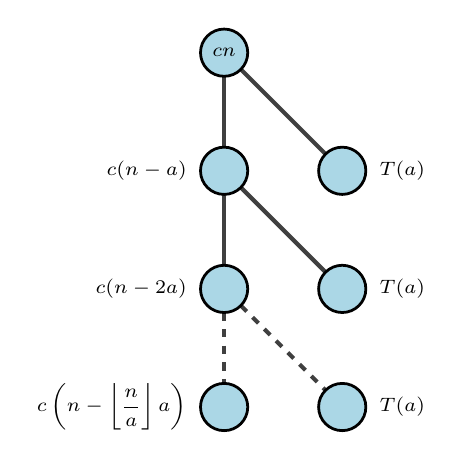
\begin{tikzpicture}
			\Vertex[label = $cn$]{0}
			\Vertex[label = $c(n - a)$, y = -1.5, position = left, distance = 0.5mm]{1}
			\Vertex[label = $T(a)$, x = 1.5, y = -1.5, position = right, distance = 0.5mm]{2}
			\Vertex[label = $c(n - 2a)$, y = -3, position = left, distance = 0.5mm]{3}
			\Vertex[label = $T(a)$, x = 1.5, y = -3, position = right, distance = 0.5mm]{4}
			\Vertex[label = $c\left(n - \left\lfloor\dfrac{n}{a}\right\rfloor a\right)$, y = -4.5, position = left, distance = 0.5mm]{5}
			\Vertex[label = $T(a)$, x = 1.5, y = -4.5, position = right, distance = 0.5mm]{6}
			\Edge(0)(1)
			\Edge(0)(2)
			\Edge(1)(3)
			\Edge(1)(4)
			\Edge[style = {dashed}](3)(5)
			\Edge[style = {dashed}](3)(6)
		\end{tikzpicture}\newline
		易知递归树一共有$\left\lfloor\dfrac{n}{a}\right\rfloor$层, 故总复杂度为:\newline
		$
		\begin{aligned}
			T(n) &= nT(a) + \sum\limits_{k = 0}^{\lfloor n/a\rfloor}c(n - ka) \\
			&= cn(\lfloor n/a\rfloor + 1) - ca\dfrac{\lfloor n/a\rfloor\left(\lfloor n/a\rfloor + 1\right)}{2} + nT(a)
		\end{aligned}
		$\newline
		因为$\lfloor n/a\rfloor = \Theta(n)$, 故$T(n) = \Theta(n^2)$
	\end{solution}
	\begin{solution}\textnormal{\textbf{6.}}
		\textbf{a.}本题中$a = 2, b = 4$, 则$\log_ba = \dfrac{1}{2}$, 故$n^{\log_ba} = \sqrt{n} = f(n)$. 即$f(n) = \Theta(\sqrt{n})$\newline
		故由主方法可得:$T(n) = \Theta(\sqrt{n}\lg n)$.\newline
		\textbf{b.}本题中$a = 2, b = 4$, 则$\log_ba = \dfrac{1}{2}$, 故$n^{\log_ba} = \sqrt{n}$.\newline
		故存在正常数$\varepsilon = \dfrac{1}{2}$, 有$f(n) = \Omega(n^{\log_ba + \varepsilon}) = \Omega(n)$.\newline
		且存在$c = \dfrac{1}{2} < 1$, 使得对于所有足够大的$n$均有$af(n/b) = \dfrac{n^2}{8} \leq \dfrac{n^2}{2} = cf(n)$.\newline
		故由主方法可知:$f(n) = \Theta(f(n)) = \Theta(n^2)$
	\end{solution}
	\begin{solution}\textnormal{\textbf{7.}}
		不能使用主方法.\newline
		此时$f(n) = n^2\lg n$, $n^{\log_ba} = n^2$. 因为对于任何正常数$\alpha$, 有$\lim\limits_{n \to +\infty}\dfrac{\lg n}{n^{\alpha}} = 0$, 显然此时不存在正常数$\varepsilon$, 使得$f(n) = \Theta(n^{2 - \varepsilon})$或是$f(n) = \Theta(n^{2 + \varepsilon})$. 因此无法使用主方法.\newline
		此时应使用递归树或是代入法来进行求解.\newline
		下面给出代入法证明$T(n) = O(n^{2}\lg^2 n)$.\newline
		若对于所有$2 \leq k < n$, 有$T(k) \leq k^2\lg^2 k$, 则当$k = n$时, 有:\newline
		$
		\begin{aligned}
			T(n) &= 4T(n/2) + n^2\lg n \\
			&\leq 4 \times \left(\left(\dfrac{n}{2}\right)^2\lg^2\dfrac{n}{2}\right) + n^2\lg n \\
			&= n^2(\lg n - 1)^2 + n^2\lg n \\
			&= n^2\lg^2n + n^2(1 - \lg n) \leq n^2\lg^2n
		\end{aligned}
		$\newline
		即存在正常数$c = 1$, 使得存在$n_0 = 2$, 当$n > n_0$时, 有$0 \leq T(n) \leq n^2\lg^2n$\newline
		故$T(n) = O(n^2\lg^2n)$
	\end{solution}
	$	%在数学环境中使用矩阵, 矩阵环境中不用使用数学环境 $$
	\begin{pmatrix}
		\dfrac{\partial y_1}{\partial x_1} & \cdots & \dfrac{\partial y_n}{\partial x_1} \\
		\vdots & \ddots & \vdots \\
		\dfrac{\partial y_1}{\partial x_n} & \cdots & \dfrac{\partial y_n}{\partial x_n}
	\end{pmatrix}
	$
\end{document}









